\documentclass{article}

\usepackage{graphicx}
\usepackage{listings}
\usepackage{float}

\usepackage{xepersian}
\settextfont{XB Zar}

\title{تمرین سری اول درس سیستم‌های عامل پیشرفته}
\author{پارسا محمدیان -- 98102284}
\date{\today}

\begin{document}
\maketitle

\section*{تئوری}
\section{}
از آنجایی که در مجموع 
$$
4 \times 20 \times 2 = 160
$$
ریسمان می‌تواند در سیستم به صورت همزمان اجرا شود، این ۲۵۶ ریسمان باید در 
دو نوبت اجرا شوند. در هر نوبت آدرس‌هایی که 
\lr{allocate}
می‌شوند در 
\lr{TLB}
ذخیره می‌شوند و سپس با 
\lr{TLB Shootdown IPI}
پاک می‌شوند. تعداد این 
\lr{TLB Shootdown IPI}ها 
باید برابر تعداد 
\lr{deallocate}ها 
باشد یعنی برابر با عدد زیر.
$$
10^6 \times 256 = 2^20 \times 2^8 = 2^{28}
$$
برای کاهش این عدد می‌توانیم قبل از 
\lr{deallocate}
کردن،‌ یک دور 
\lr{instruction}
مربوط به 
\lr{TLB Shootdown}
را اجرا می‌کنیم و سپس حافظه‌های گرفته شده را 
\lr{deallocate}
می‌کنیم. اینگونه فاکتور تعداد 
\lr{deallocate}ها 
از ضرب بالا حذف می‌شوند.

\section*{عملی}
\setcounter{section}{0}
\section{}
\subsection{}
\subsubsection{}
کد مربوط به این بخش در فایل 
\lr{1.1.c}
موجود است. همچنین اسکریپت اجرای آن در فایل
\lr{1.1.sh}
قرار دارد.

در تصویر زیر مشاهده می‌کنیم که اسکریپت اجرا شده است.
خروجی کامل اسکریپت را در ادامه می‌بینیم.

\begin{figure}[H]
\centering
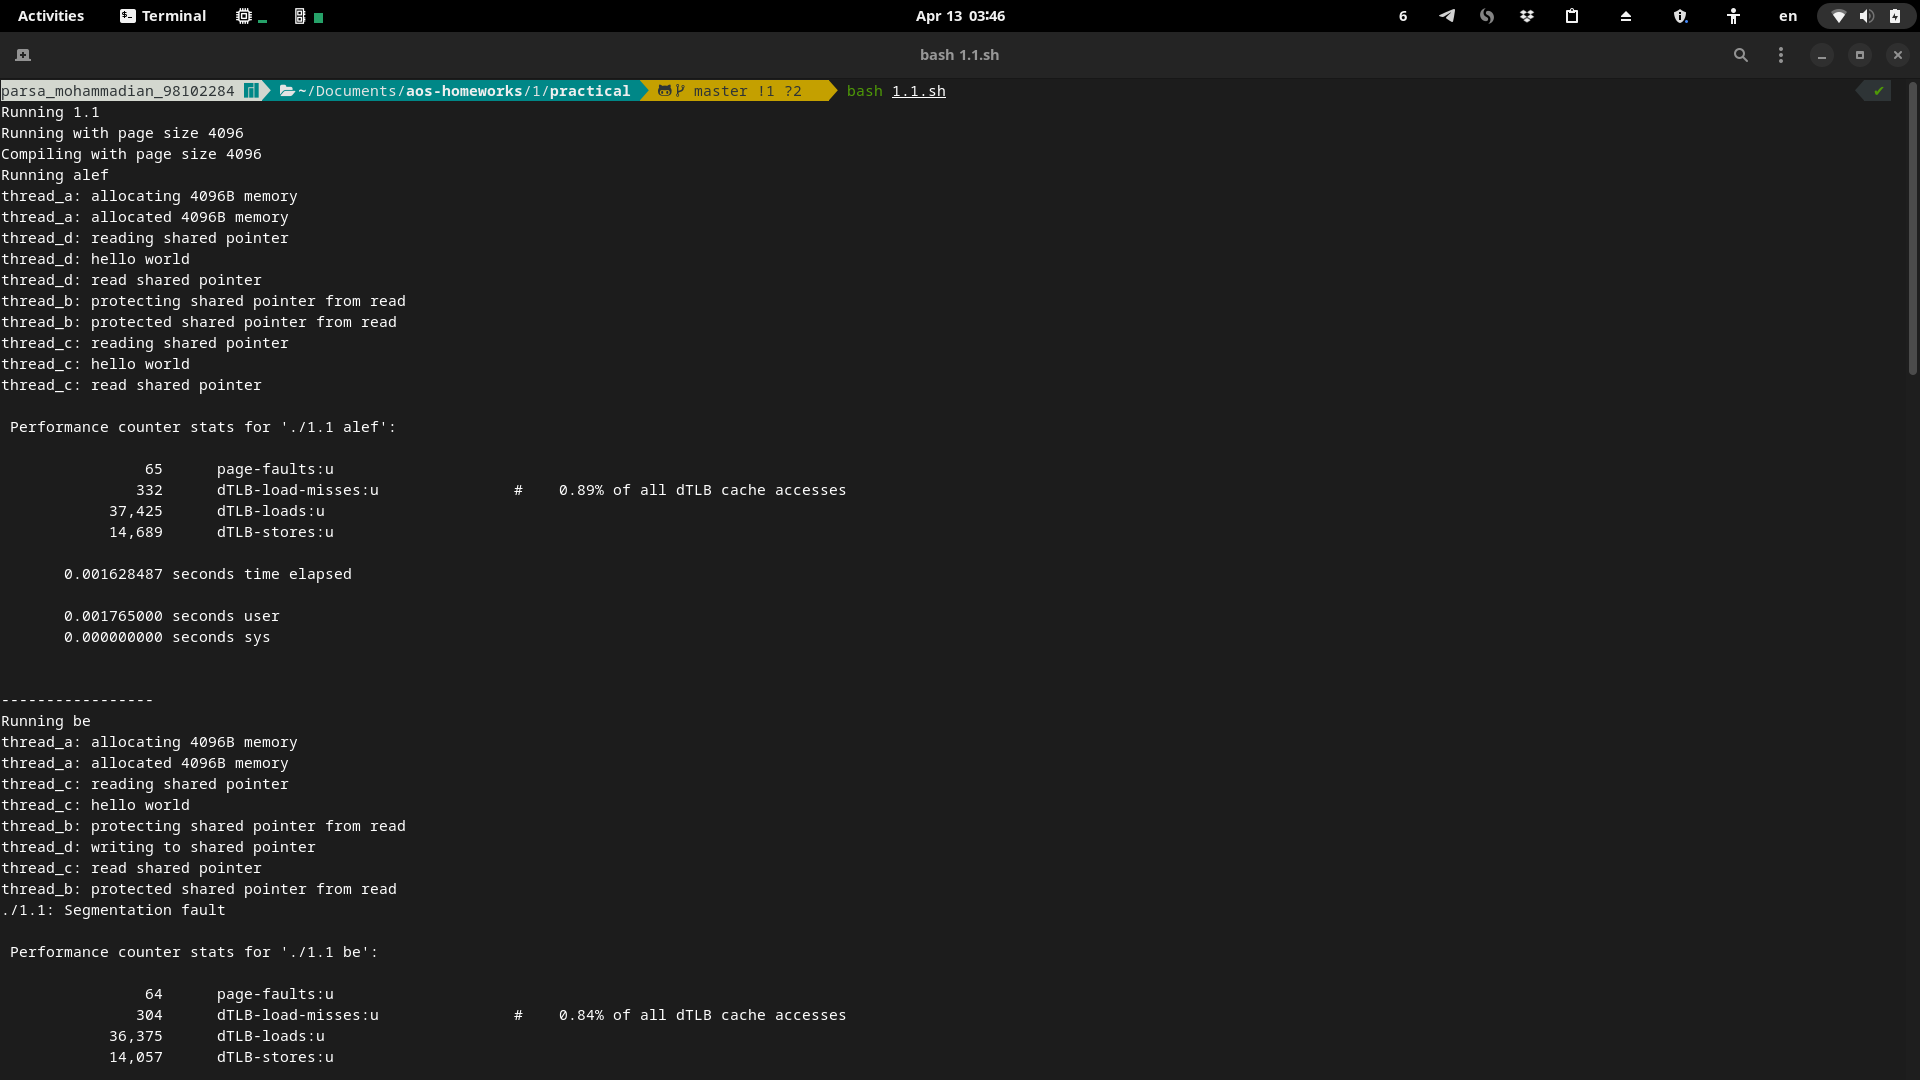
\includegraphics[width=\textwidth]{1.1.png}
\caption{خروجی اجرای اسکریپت}
\label{fig:1.1}
\end{figure}

\begin{latin}
\begin{lstlisting}
Running 1.1
Running with page size 4096
Compiling with page size 4096
Running alef
thread_a: allocating 4096B memory
thread_a: allocated 4096B memory
thread_d: reading shared pointer
thread_d: hello world
thread_d: read shared pointer
thread_b: protecting shared pointer from read
thread_b: protected shared pointer from read
thread_c: reading shared pointer
thread_c: hello world
thread_c: read shared pointer

 Performance counter stats for './1.1 alef':

                65      page-faults:u                                                         
               332      dTLB-load-misses:u               #    0.89% of all dTLB cache accesses
            37,425      dTLB-loads:u                                                          
            14,689      dTLB-stores:u                                                         

       0.001628487 seconds time elapsed

       0.001765000 seconds user
       0.000000000 seconds sys


-----------------
Running be
thread_a: allocating 4096B memory
thread_a: allocated 4096B memory
thread_c: reading shared pointer
thread_c: hello world
thread_b: protecting shared pointer from read
thread_d: writing to shared pointer
thread_c: read shared pointer
thread_b: protected shared pointer from read
./1.1: Segmentation fault

 Performance counter stats for './1.1 be':

                64      page-faults:u                                                         
               304      dTLB-load-misses:u               #    0.84% of all dTLB cache accesses
            36,375      dTLB-loads:u                                                          
            14,057      dTLB-stores:u                                                         

       0.158606399 seconds time elapsed

       0.000000000 seconds user
       0.012408000 seconds sys


-----------------
Running jim
thread_a: allocating 4096B memory
thread_a: allocated 4096B memory
thread_d: writing to shared pointer
thread_d: wrote to shared pointer
thread_b: protecting shared pointer from read
thread_c: writing to shared pointer
thread_b: protected shared pointer from read
./1.1: Segmentation fault

 Performance counter stats for './1.1 jim':

                62      page-faults:u                                                         
               332      dTLB-load-misses:u               #    0.92% of all dTLB cache accesses
            36,252      dTLB-loads:u                                                          
            13,943      dTLB-stores:u                                                         

       0.124682004 seconds time elapsed

       0.000000000 seconds user
       0.009419000 seconds sys


-----------------
Running with page size 1024
Compiling with page size 1024
Running alef
thread_a: allocating 1024B memory
thread_a: allocated 1024B memory
thread_d: reading shared pointer
thread_d: hello world
thread_d: read shared pointer
thread_b: protecting shared pointer from read
thread_c: reading shared pointer
thread_c: hello world
thread_c: read shared pointer
thread_b: protected shared pointer from read

 Performance counter stats for './1.1 alef':

                63      page-faults:u                                                         
               354      dTLB-load-misses:u               #    0.95% of all dTLB cache accesses
            37,429      dTLB-loads:u                                                          
            14,711      dTLB-stores:u                                                         

       0.001630073 seconds time elapsed

       0.000000000 seconds user
       0.001795000 seconds sys


-----------------
Running be
thread_a: allocating 1024B memory
thread_a: allocated 1024B memory
thread_d: writing to shared pointer
thread_d: wrote to shared pointer
thread_b: protecting shared pointer from read
thread_b: protected shared pointer from read
thread_c: reading shared pointer
thread_c: thread_d was here
thread_c: read shared pointer

 Performance counter stats for './1.1 be':

                64      page-faults:u                                                         
               331      dTLB-load-misses:u               #    0.89% of all dTLB cache accesses
            37,251      dTLB-loads:u                                                          
            14,555      dTLB-stores:u                                                         

       0.001191988 seconds time elapsed

       0.000000000 seconds user
       0.001367000 seconds sys


-----------------
Running jim
thread_a: allocating 1024B memory
thread_a: allocated 1024B memory
thread_c: writing to shared pointer
thread_c: wrote to shared pointer
thread_b: protecting shared pointer from read
thread_b: protected shared pointer from read
thread_d: writing to shared pointer
./1.1: Segmentation fault

 Performance counter stats for './1.1 jim':

                67      page-faults:u                                                         
               324      dTLB-load-misses:u               #    0.90% of all dTLB cache accesses
            36,151      dTLB-loads:u                                                          
            13,968      dTLB-stores:u                                                         

       0.124665005 seconds time elapsed

       0.000000000 seconds user
       0.008697000 seconds sys
\end{lstlisting}
\end{latin}
\subsubsection{}
اعداد زیر از خروجی که در بالا آمده است به دست آمده‌اند. 
\begin{latin}
page-faults: 65, 64, 62 \\
dTLB-load-misses: 332, 304, 332 \\
dTLB-loads: 37425, 36375, 36252 \\
dTLB-stores: 14689, 14057, 13943
\end{latin}
با توجه به این اعداد،‌ 
\lr{page fault}ها
کم شده‌اند و عملیات‌های مربوط به 
\lr{TLB} 
نیز کم شده است. ولی با این حال 
\lr{miss}
ها تفاوت معناداری نکرده‌اند. 

\subsubsection{}
در این سه حالت، در حالت الف امکان ندارد 
\lr{page fault}
رخ بدهد. در حالت ب امکان رخ دادن 
\lr{page fault}
وجود دارد و این بستگی به این دارد که ریسمان 
\lr{D}
زودتر اجرا شود یا ریسمان 
\lr{B}.
در حالت ج هم همانند حالت ب این امکان وجود دارد و عملا 
\lr{race condition}
بین سه ریسمان 
\lr{B}،
\lr{C} و 
\lr{D}
به وجود می‌آید.

\subsubsection{}
برای شماره اول، خروی 
\lr{perf}
در همان قسمت و در خروجی اجرای اسکریپت آمده است. 

برای شماره دوم اعداد را از خروجی همانند قبل درمیاوریم.
\begin{latin}
page-faults: 63, 64, 67 \\
dTLB-load-misses: 354, 331, 324 \\
dTLB-loads: 37429, 37251, 36151 \\
dTLB-stores: 14711, 14555, 13968
\end{latin}
با توجه به این اعداد،‌ تعداد 
\lr{page fault}ها
بیشتر شده‌اند و آمار مربوط به 
\lr{TLB}
کاهش پیدا کرده‌اند. 

برای شماره سوم کد کاملا مانند حالت قبل که صفحات ۴ کیلوبایتی است 
عمل می‌کند. 
\subsection{}
\subsubsection{}
کد مربوط به این بخش در فایل 
\lr{1.2.c}
وجود دارد. همچنین اسکریپت مربوط به اجرای این کد در فایل 
\lr{1.2.sh}
موجود می‌باشد. در عکس زیر اجرا شدن این اسکریپت را مشاهده میکنیم. خروجی مربوط 
به آن در ادامه به صورت کامل آمده است. 

\begin{figure}[H]
   \centering
   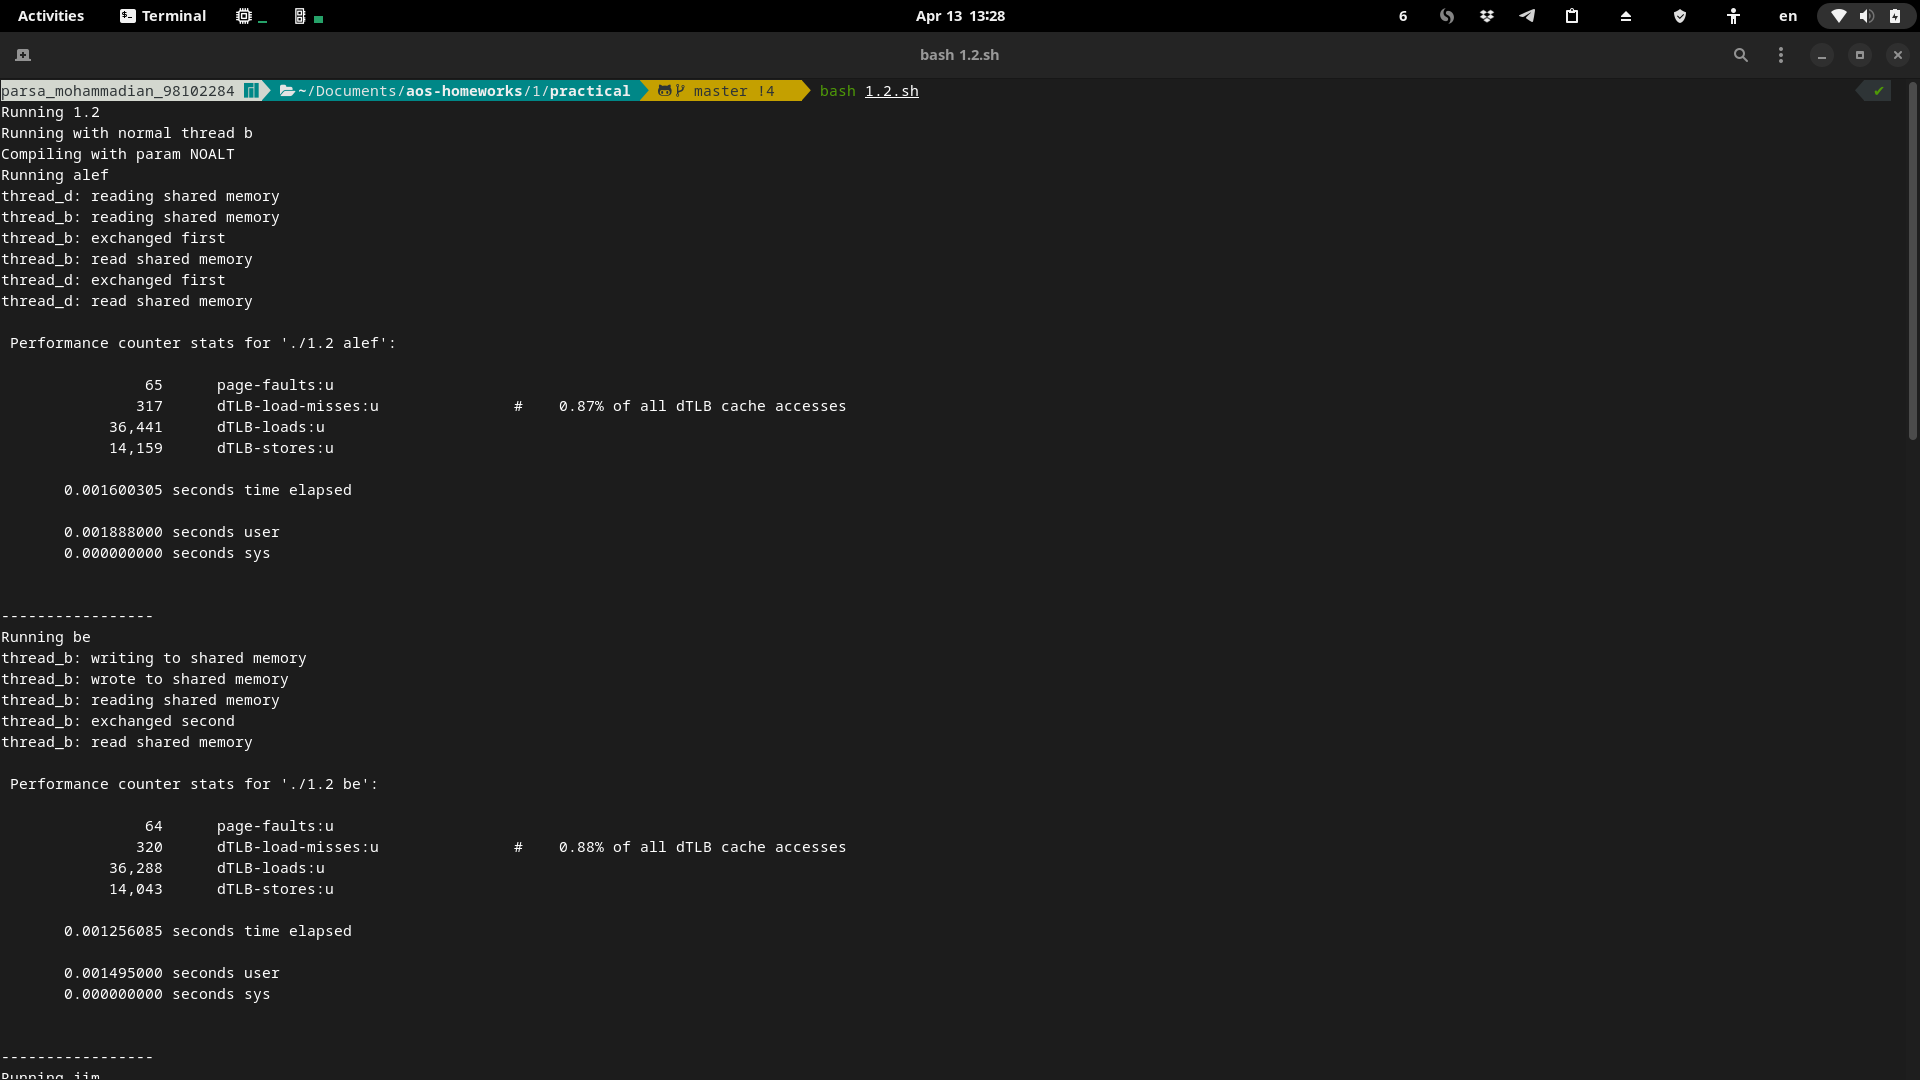
\includegraphics[width=\linewidth]{1.2.png}
   \caption{اجرا کردن اسکریپت}
\end{figure}

\begin{latin}
\begin{lstlisting}
Running 1.2
Running with normal thread b
Compiling with param NOALT
Running alef
thread_d: reading shared memory
thread_b: reading shared memory
thread_b: exchanged first
thread_b: read shared memory
thread_d: exchanged first
thread_d: read shared memory

 Performance counter stats for './1.2 alef':

                65      page-faults:u                                                         
               317      dTLB-load-misses:u               #    0.87% of all dTLB cache accesses
            36,441      dTLB-loads:u                                                          
            14,159      dTLB-stores:u                                                         

       0.001600305 seconds time elapsed

       0.001888000 seconds user
       0.000000000 seconds sys


-----------------
Running be
thread_b: writing to shared memory
thread_b: wrote to shared memory
thread_b: reading shared memory
thread_b: exchanged second
thread_b: read shared memory

 Performance counter stats for './1.2 be':

                64      page-faults:u                                                         
               320      dTLB-load-misses:u               #    0.88% of all dTLB cache accesses
            36,288      dTLB-loads:u                                                          
            14,043      dTLB-stores:u                                                         

       0.001256085 seconds time elapsed

       0.001495000 seconds user
       0.000000000 seconds sys


-----------------
Running jim
thread_b: writing to shared memory
thread_b: wrote to shared memory
thread_c: writing to shared memory
thread_c: wrote to shared memory

 Performance counter stats for './1.2 jim':

                63      page-faults:u                                                         
               284      dTLB-load-misses:u               #    0.79% of all dTLB cache accesses
            35,948      dTLB-loads:u                                                          
            13,807      dTLB-stores:u                                                         

       0.000940042 seconds time elapsed

       0.001195000 seconds user
       0.000000000 seconds sys


-----------------
Running with alternative thread b implementation
Compiling with param ALT
Running alef
thread_d: reading shared memory
./1.2: Segmentation fault

 Performance counter stats for './1.2 alef':

                64      page-faults:u                                                         
               279      dTLB-load-misses:u               #    0.80% of all dTLB cache accesses
            35,031      dTLB-loads:u                                                          
            13,388      dTLB-stores:u                                                         

       0.132951991 seconds time elapsed

       0.000000000 seconds user
       0.009916000 seconds sys


-----------------
Running be
thread_b: writing to shared memory
thread_b: wrote to shared memory
thread_b: reading shared memory
thread_b: thread b was here
thread_b: read shared memory

 Performance counter stats for './1.2 be':

                64      page-faults:u                                                         
               308      dTLB-load-misses:u               #    0.84% of all dTLB cache accesses
            36,506      dTLB-loads:u                                                          
            14,122      dTLB-stores:u                                                         

       0.001034783 seconds time elapsed

       0.001186000 seconds user
       0.000000000 seconds sys


-----------------
Running jim
thread_b: writing to shared memory
thread_b: wrote to shared memory
thread_c: writing to shared memory
./1.2: Segmentation fault

 Performance counter stats for './1.2 jim':

                62      page-faults:u                                                         
               292      dTLB-load-misses:u               #    0.83% of all dTLB cache accesses
            35,269      dTLB-loads:u                                                          
            13,416      dTLB-stores:u                                                         

       0.112482720 seconds time elapsed

       0.000000000 seconds user
       0.009095000 seconds sys   
\end{lstlisting}
\end{latin}
\subsubsection{}
از خروجی قسمت بالا اعداد زیر را بدست می‌آوریم.
\begin{latin}
page-faults: 65, 64, 63 \\
dTLB-load-misses: 317, 320, 284 \\
dTLB-loads: 36441, 36288, 35948 \\
dTLB-stores: 14159, 14043, 13807
\end{latin}
با توجه به این اعداد تعداد 
\lr{page fault}ها
کاهش پیدا کرده است ولی روند مشخصی در عملیات‌های مربوط به 
\lr{TLB}
مشاهده نمی‌شود. 

\subsubsection{}
خروجی خواسته شده در همان خروجی اسکریپت قسمت اول آورده شده است. اعداد زیر را برای 
تحلیل از خروجی بالا استراج می‌کنیم. 
\begin{latin}
page-faults: 64, 64, 62 \\
dTLB-load-misses: 279, 308, 292 \\
dTLB-loads: 35031, 36506, 35269 \\
dTLB-stores: 13388, 14122, 13416
\end{latin}
الگو این اعداد همانند اعدادی هستند که در اجرای قبلی دیده شدند. پس می‌توانیم نتیجه بگیریم 
\lr{munmap} 
کردن فرقی با 
\lr{mmap}
کردن جای جدید در حافظه ندارد. 

\subsection{}
\subsubsection{}
کد مربوط به این بخش در فایل 
\lr{1.3.c}
قرار دارد. همچنین اسکریپت اجرای آن در فایل 
\lr{1.3.sh}
قرار دارد.

در تصویر 
\ref{fig:1.3}
مشاهده می‌کنیم که این اسکریپت اجرا شده است. 
خروجی آن را در ادامه می‌بینیم. 

\begin{figure}[H]
\centering
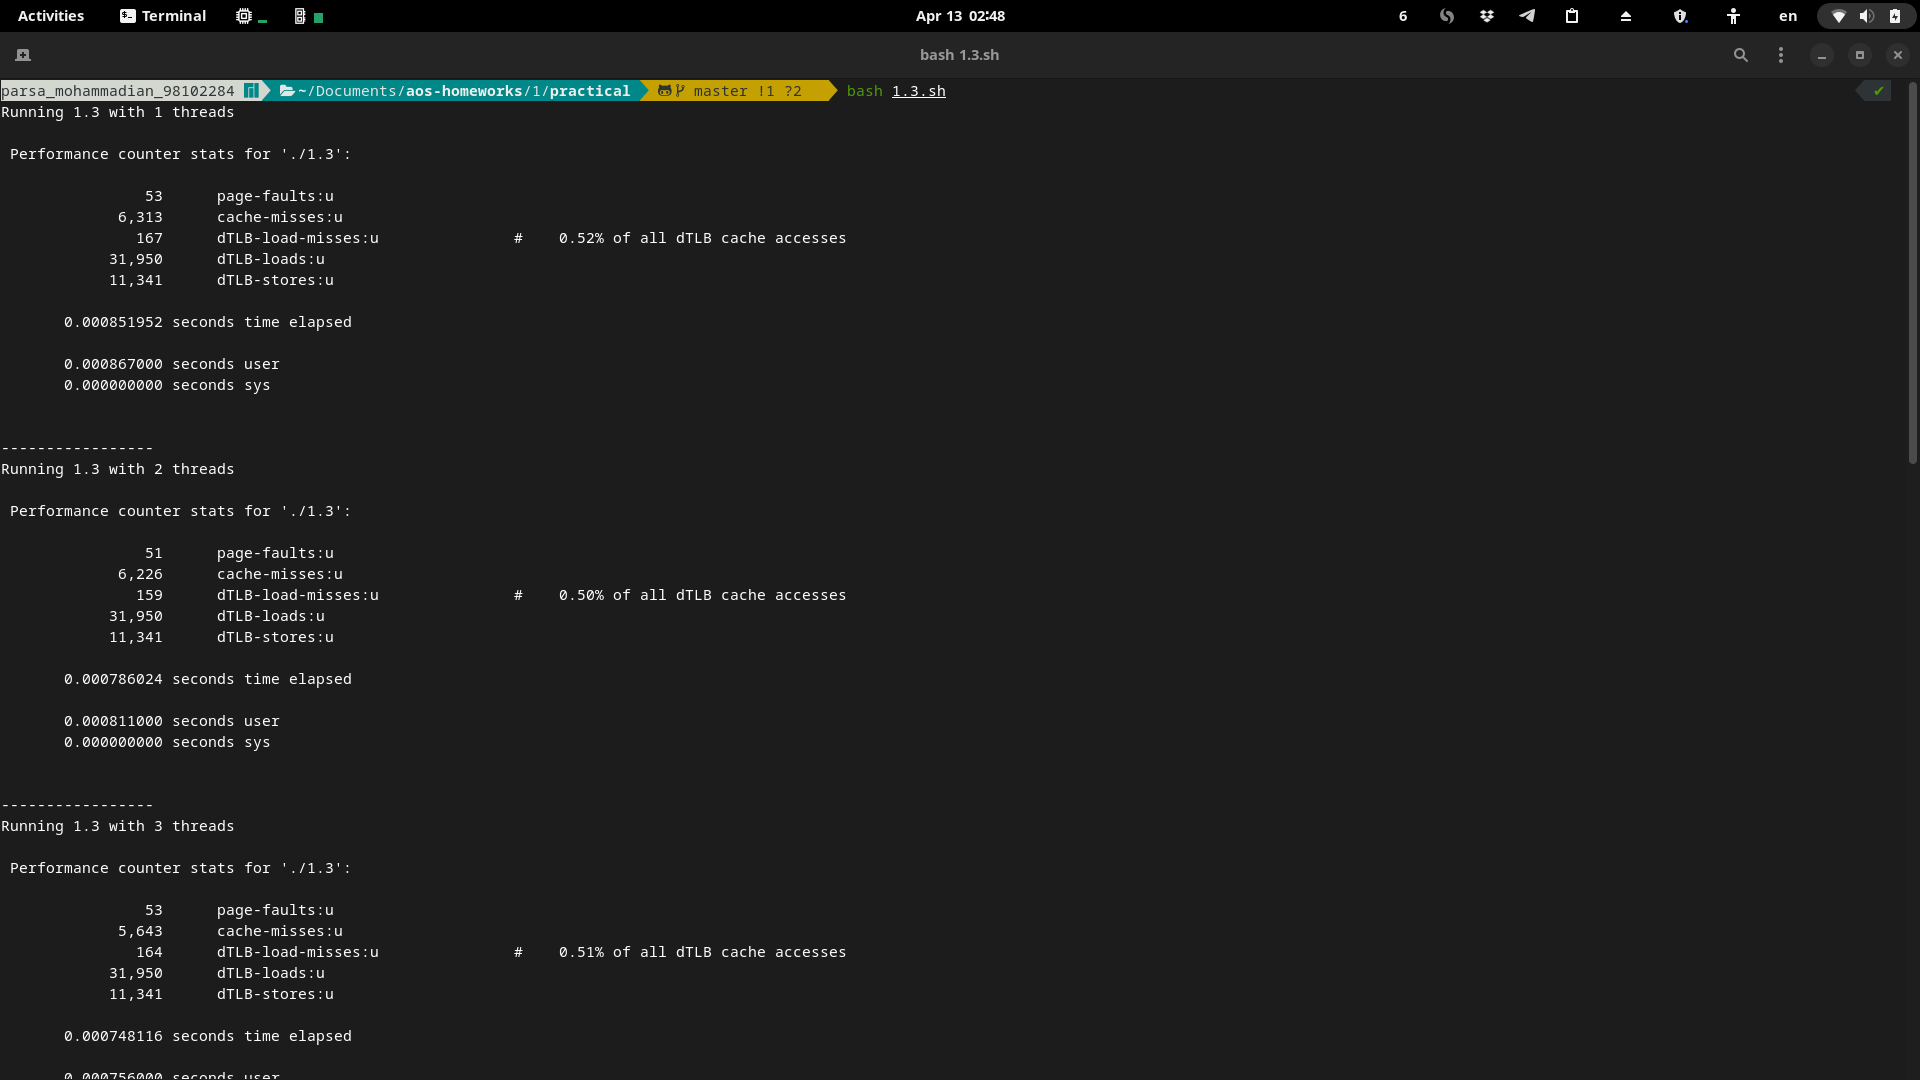
\includegraphics[width=\textwidth]{1.3.png}
\caption{خروجی اجرای اسکریپت}
\label{fig:1.3}
\end{figure}

\begin{latin}
\begin{lstlisting}
Running 1.3 with 1 threads

 Performance counter stats for './1.3':

                53      page-faults:u                                                         
             6,313      cache-misses:u                                                        
               167      dTLB-load-misses:u               #    0.52% of all dTLB cache accesses
            31,950      dTLB-loads:u                                                          
            11,341      dTLB-stores:u                                                         

       0.000851952 seconds time elapsed

       0.000867000 seconds user
       0.000000000 seconds sys


-----------------
Running 1.3 with 2 threads

 Performance counter stats for './1.3':

                51      page-faults:u                                                         
             6,226      cache-misses:u                                                        
               159      dTLB-load-misses:u               #    0.50% of all dTLB cache accesses
            31,950      dTLB-loads:u                                                          
            11,341      dTLB-stores:u                                                         

       0.000786024 seconds time elapsed

       0.000811000 seconds user
       0.000000000 seconds sys


-----------------
Running 1.3 with 3 threads

 Performance counter stats for './1.3':

                53      page-faults:u                                                         
             5,643      cache-misses:u                                                        
               164      dTLB-load-misses:u               #    0.51% of all dTLB cache accesses
            31,950      dTLB-loads:u                                                          
            11,341      dTLB-stores:u                                                         

       0.000748116 seconds time elapsed

       0.000756000 seconds user
       0.000000000 seconds sys


-----------------
Running 1.3 with 4 threads

 Performance counter stats for './1.3':

                53      page-faults:u                                                         
             5,510      cache-misses:u                                                        
               157      dTLB-load-misses:u               #    0.49% of all dTLB cache accesses
            31,921      dTLB-loads:u                                                          
            11,341      dTLB-stores:u                                                         

       0.001029236 seconds time elapsed

       0.001070000 seconds user
       0.000000000 seconds sys


-----------------
Running 1.3 with 5 threads

 Performance counter stats for './1.3':

                52      page-faults:u                                                         
             5,868      cache-misses:u                                                        
               159      dTLB-load-misses:u               #    0.50% of all dTLB cache accesses
            31,950      dTLB-loads:u                                                          
            11,341      dTLB-stores:u                                                         

       0.000757058 seconds time elapsed

       0.000747000 seconds user
       0.000000000 seconds sys


-----------------
Running 1.3 with 6 threads

 Performance counter stats for './1.3':

                51      page-faults:u                                                         
             6,439      cache-misses:u                                                        
               162      dTLB-load-misses:u               #    0.51% of all dTLB cache accesses
            31,950      dTLB-loads:u                                                          
            11,341      dTLB-stores:u                                                         

       0.000781736 seconds time elapsed

       0.000827000 seconds user
       0.000000000 seconds sys


-----------------
Running 1.3 with 7 threads

 Performance counter stats for './1.3':

                52      page-faults:u                                                         
             3,688      cache-misses:u                                                        
               161      dTLB-load-misses:u               #    0.50% of all dTLB cache accesses
            31,950      dTLB-loads:u                                                          
            11,341      dTLB-stores:u                                                         

       0.000675503 seconds time elapsed

       0.000679000 seconds user
       0.000000000 seconds sys


----------------- 
\end{lstlisting}
\end{latin}

\subsubsection{}
کد مربوط به این نمودار و نمودار قسمت بعد در فایل 
\lr{1.3.py}
موجود است. 

تصویر این نمودار در اینجا قابل مشاهده است. 
\begin{figure}[H]
\centering
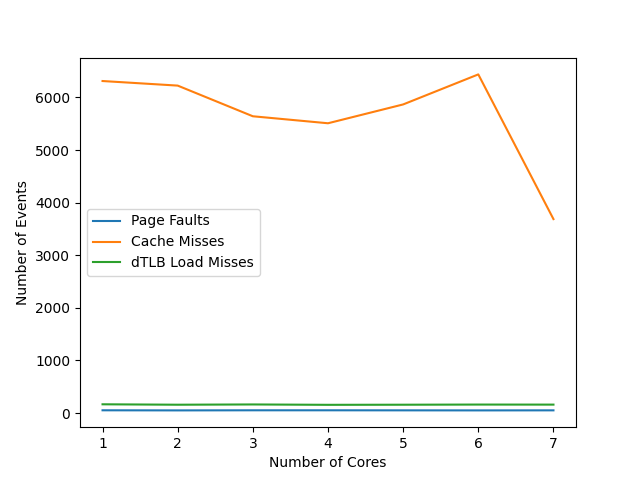
\includegraphics[width=\textwidth]{1.3-plot-1.png}
\caption{نمودار تاثیر تعداد ریسمان‌ها بر پارامترها}
\end{figure}

\subsubsection{}
نمودار خواسته شده در شکل زیر قابل مشاهده است. 

\begin{figure}[H]
\centering
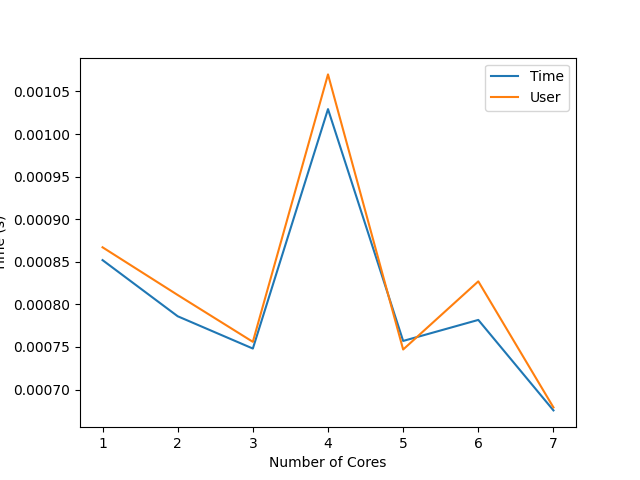
\includegraphics[width=\textwidth]{1.3-plot-2.png}
\caption{نمودار تاثیر تعداد ریسمان‌ها بر تاخیر زمان اجرای برنامه}
\end{figure}

\end{document}